\documentclass[12pt]{article}

\usepackage{amsmath}
\usepackage{amssymb}
\usepackage{amsfonts}
\usepackage{polski}
\usepackage{verbatim}
\usepackage[utf8]{inputenc}
\usepackage[polish]{babel}
\usepackage[T1]{fontenc}
\usepackage{graphicx}
\usepackage{caption}
\usepackage{enumitem}
\usepackage{hyperref}
\usepackage{natbib}
\usepackage{graphicx}
\usepackage{datetime}
\usepackage{multirow}
\usepackage{array}
\newdateformat{mydate}{\twodigit{\THEDAY}.\twodigit{\THEMONTH}.\THEYEAR r.}
\usepackage{enumitem}
\usepackage{footnote}
\setlist{
	noitemsep,
	listparindent=\parindent,
	parsep=0pt,
}
\makesavenoteenv{tabular}
\makesavenoteenv{table}

\usepackage{xparse}

\textheight 23.2 cm
\textwidth 6.0 in
\hoffset = -0.5 in
\voffset = -2.4 cm

\begin{document}

\begin{titlepage}
	\begin{flushright}
		{\mydate\today}\\
	\end{flushright}
	\vskip30ex

	\begin{center}
		\Large {\bf{
				System do zdalnej pracy w środowisku graficznym wykorzystujący maszyny wirtualne QEMU z akceleracja sprzętową\\
			}}
		\vskip2ex
		\bf{Sprawozdanie z testów\\}
		\vskip2ex
		\small { Autorzy: Krzysztof Smogór, Piotr Widomski\\  }
		\small { Promotor: Dr inż. Marek Kozłowski\\ }
	\end{center}
\end{titlepage}

\tableofcontents

\newpage

\section{Testy jednostkowe}

\section{Testy integracyjne}

\subsection {Testy integracji z libvirtem oraz vagrantem}

Przy integracji systemu z libvirtem oraz vagrantem musielismy sprawdzic następujące funkcjonalności:
\begin{enumerate}
	\item Włączanie maszyn poprzez vagranta
	\item Wyłączanie maszyn poprzez vagranta
	\item Sprawdzanie czy maszyna jest uruchomiona poprzez libvirta
	\item Pobranie adresu IP uruchomionej maszyny wirtualnej
\end{enumerate}

Aby testy miały sens potrzebowaliśmy konfiguracji XML do tworzenia maszyn \textit{transient} oraz gotowego lekkiego vagrant-boxa przy tworzeniu maszyn \textit{persistence}.
Przy testach libvirta wykorzystaliśmy obraz live ArchLinuxa, którego uruchamiamy w minimalnie przygotowanej konfiguracji.
Do testów vagranta skorzystaliśmy z lekkiego obrazu "generic/alpine38".
Przy testach konfiguracji sieciowej utworzyliśmy bridge sieciowy, który jest uwzględniony w konfiguracji uruchamianych maszyn wirtualnych.

Aby upewnić się, że wszystko działa prawidłowo skorzystaliśmy z mechaniki testów jednostkowych NUnit przy jednocześnie uruchomionym daemonie libvirta.

\begin{figure}[!h]
	\centering
	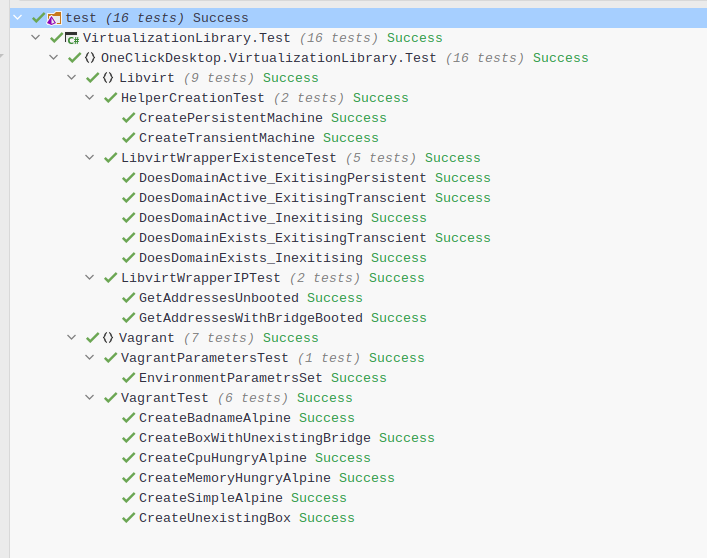
\includegraphics[width=0.7\linewidth]{res/virtsrvlib-test}
	\caption{Lista testów sprawdzających integrację z libvirtem i vagrantem}
	\label{fig:virtsrvlib-test}
\end{figure}

\subsection{Testy integracyjne z RabbitMQ}
Podczas tworzenia projektu wydzieliliśmy osobny moduł, którego celem jest obłożenie biblioteki API RabbitMQ w interfejs, który umożliwi wygodne użytkowanie brokera z poziomu głównych modułów systemu. Jako iż biblioteka ta nie posiada wewnętrznej logiki, a jedynie wywołuje odpowiednie funkcje brokera wiadomości, przetestowana została z użyciem testów integracyjnych. Testowana funkcjonalność obejmowała:
\begin{enumerate}
	\item Tworzenie punktów wymiany (exchange)
	\item Tworzenie kolejek i podłączanie ich do punktów wymiany
	\item Wysyłanie i odbieranie wiadomości (wraz z zaimplementowanym mechanizmem deserializacji)
	\item Wysyłanie wiadomości do konkretnych odbiorców
	\item Wykrywanie braku odbiorców
\end{enumerate}

W tym celu wykorzystaliśmy metodę analogiczną do testów z libvirtem, czyli mechaniki testów jednostkowych NUnit przy jednocześnie uruchomionym brokerze RabbitMQ.

\section{Testy E2E}
Aplikacja kliencka oraz panel administratora posiadają proste testy E2E, z wykorzystaniem platformy Cypress, spełniające równocześnie po części rolę testów UI. Testy te skupiają się na pojedynczych ekranach aplikacji oraz jej działaniu z perspektywy użytkownika.

Planujemy dodanie testów E2E realizujących wielokrokowe scenariusze testowe, zaczynające się od zalogowania do aplikacji.

\section{Scenariusze akceptacyjne}

\section{Aktualny stan testów}
Na ten moment następujące elementy systemu posiadają testy automatyczne (wraz z typem testów):
\begin{itemize}
	\item Aplikacja kliencka (testy jednostkowe, UI, proste E2E)
	\item Panel administratora (testy jednostkowe, UI, proste E2E)
	\item Moduł serwera wirtualizacji (testy integracyjne libvirt)
	\item Biblioteka modelu systemu (testy jednostkowe)
	\item Biblioteka brokera wiadomości (testy integracyjne)
\end{itemize}
Testy jednostkowe do modułów:
\begin{itemize}
	\item Nadzorca
	\item Serwer wirtualizacji
\end{itemize}
są w trakcie powstawania.
Powstaną również testy E2E, które również realizować część scenariuszy akceptacyjnych.

\end{document}